% ------------------------------------------------------------------------------
% TYPO3 CMS 6.2 LTS - What's New - Chapter "Install Tool" (French version)
%
% @author	Paul Blondiaux <pblondiaux@sodifrance.fr>
% @author	Philippe Herault <philippe.herault@plan-net.fr>
% @license	Creative Commons BY-NC-SA 3.0
% @link		http://typo3.org/download/release-notes/whats-new/
% @language	French
% ------------------------------------------------------------------------------
% Chapitre : Install Tool
% ------------------------------------------------------------------------------

\section{Install Tool}
\begin{frame}[fragile]
	\frametitle{Install Tool}

	\begin{center}\huge{Chapitre 1 :}\end{center}
	\begin{center}\huge{\color{typo3darkgrey}\textbf{L'Install Tool}}\end{center}

\end{frame}

% ------------------------------------------------------------------------------
% Installation
% ------------------------------------------------------------------------------

\begin{frame}[fragile]
	\frametitle{Install Tool}
	\framesubtitle{Installation (1)}

	\begin{itemize}
		\item Seul \underline{un} paquet est nécessaire pour l'installation :\newline
				\texttt{typo3\_src-6.2.x.tar.gz} (taille du fichier : approx. 20MB)
		\item Les paquets « Dummy » et « Blank » deviennent obsolètes
		\item Installation :
			\begin{itemize}
				\item Extraire le package source à la racine de votre serveur Web
				\item Créer des liens symboliques au besoin
				\item Ouvrir un navigateur et entrer l'URL de votre serveur
				\item L'installation de TYPO3 démarre l'assistant 1-2-3-4-steps
			\end{itemize}
		\item L'assistant d'installation s'assure que tous les fichiers et répertoires sont présents
	\end{itemize}

\end{frame}

% ------------------------------------------------------------------------------
% Installation
% ------------------------------------------------------------------------------

\begin{frame}[fragile]

	\frametitle{Install Tool}
	\framesubtitle{Installation (2)}

	\begin{itemize}
		\item Les fichiers nécessaires pour un paramétrage personnalisé se créent automatiquement
		\item Les liens symboliques suivants \underline{doivent} exister :

		\begin{itemize}
			\item \texttt{typo3\_src}	\tabto{2cm} (pointe sur le répertoire source de TYPO3)
			\item \texttt{typo3}		\tabto{2cm} (pointe sur le répertoire : \texttt{typo3\_src/typo3})
			\item \texttt{index.php}	\tabto{2cm} (pointe sur le fichier : \texttt{typo3\_src/index.php})
		\end{itemize}

		\item Aucun autre fichier ou répertoire n'est nécessaire pour l'installation de TYPO3!
		\item Le répertoire \texttt{t3lib} a été enlevé
		\item En savoir plus : Guide d'installation et de mise à jour de TYPO3\newline
			\url{http://docs.typo3.org/typo3cms/InstallationGuide}

	\end{itemize}

\end{frame}

% ------------------------------------------------------------------------------
% Re-Development
% ------------------------------------------------------------------------------

\begin{frame}[fragile]
	\frametitle{Install Tool}
	\framesubtitle{Re-Développement (1)}

	\begin{columns}[T]

		\begin{column}{.5\textwidth}
			\begin{itemize}
				\item Entièrement re-développé en utilisant Fluid
				\item \underline{La première} étape teste l'environnement système et liste les erreurs
				\item Les erreurs peuvent être corrigées (et re-testées) ou ignorées
				\item Une mauvaise configuration du cœur (par exemple : absence de liens symboliques) est aussi rapportée comme une erreur
			\end{itemize}
		\end{column}

		\begin{column}{.5\textwidth}
			\begin{figure}\vspace*{-0.4cm}
				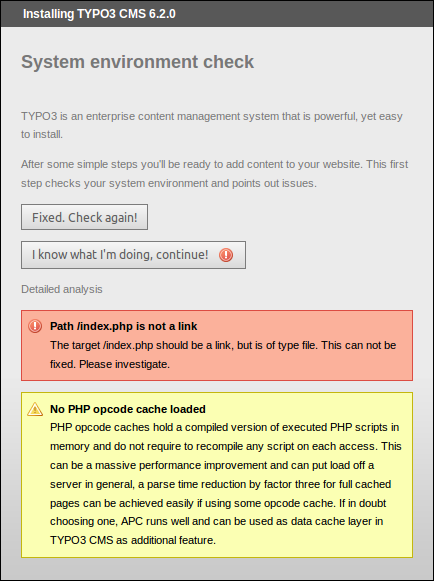
\includegraphics[width=0.8\linewidth]{Images/InstallTool/SystemEnvironmentCheck.png}
			\end{figure}
		\end{column}

	\end{columns}

\end{frame}

% ------------------------------------------------------------------------------
% Re-Development
% ------------------------------------------------------------------------------

\begin{frame}[fragile]
	\frametitle{Install Tool}
	\framesubtitle{Re-Développement (2)}

	\begin{columns}[T]

		\begin{column}{.5\textwidth}
			\begin{itemize}
				\item \underline{La Deuxième} étape permet aux utilisateurs de saisir les informations de la base de données
				\item Différents types de connexion sont possibles
					\begin{itemize}
						\item Connexion basée sur TCP/IP
						\item Connexion basée sur Socket
					\end{itemize}
				\item Des alternatives à MySQL sont possibles
			\end{itemize}
		\end{column}

		\begin{column}{.5\textwidth}
			\begin{figure}\vspace*{-0.4cm}
				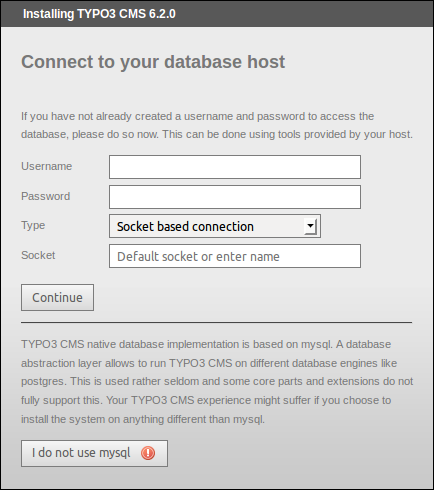
\includegraphics[width=0.8\linewidth]{Images/InstallTool/DatabaseConnectionDetails.png}
			\end{figure}
		\end{column}

	\end{columns}

\end{frame}

% ------------------------------------------------------------------------------
% Re-Development
% ------------------------------------------------------------------------------

\begin{frame}[fragile]
	\frametitle{Install Tool}
	\framesubtitle{Re-Développement (3)}

	\begin{columns}[T]

		\begin{column}{.5\textwidth}
			\begin{itemize}
				\item \underline{La Troisième} étape permet aux utilisateurs de sélectionner ou créer la base de données\newline
					(comme pour TYPO3 < 6.2)
				\item \underline{La quatrième} étape permet aux utilisateurs de saisir un mot de passe pour l'utilisateur « admin »\newline (c'est aussi le mot de passe initial de l'Install Tool) et un nom de site
			\end{itemize}
		\end{column}

		\begin{column}{.5\textwidth}
			\begin{figure}\vspace*{-0.4cm}
				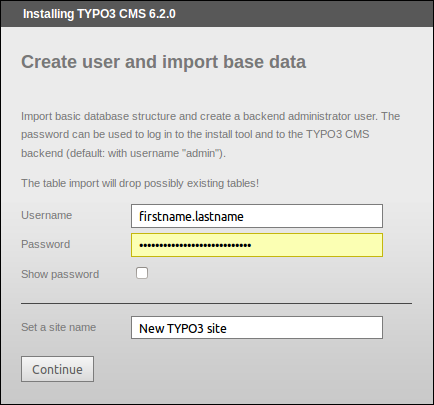
\includegraphics[width=0.8\linewidth]{Images/InstallTool/AdminPasswordAndSiteName.png}
			\end{figure}
		\end{column}

	\end{columns}

\end{frame}

% ------------------------------------------------------------------------------
% Clear All Cache
% ------------------------------------------------------------------------------

\begin{frame}[fragile]
	\frametitle{Install Tool}
	\framesubtitle{Vider tous les caches (1)}

	\begin{itemize}
		\item Une nouvelle fonction sous « Actions importantes » permet aux utilisateurs d'effacer tous les caches
		\item Cela fonctionne aussi si le cache contient du code PHP invalide\newline
			(qui peut éventuellement bloquer TYPO3 CMS)
		\item Accédez directement à l'install tool en cas d'instance TYPO3 non fonctionnelle par l'URL : \texttt{http://example.com/typo3/install}
	\end{itemize}

	\begin{columns}[T]
		\begin{column}{.3\textwidth}
			\begin{figure}\vspace*{-0.4cm}
				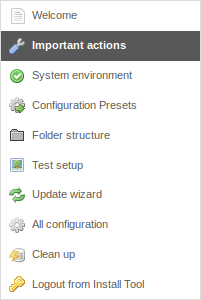
\includegraphics[width=0.7\linewidth]{Images/InstallTool/ImportantActions.png}
			\end{figure}
		\end{column}
		\begin{column}{.7\textwidth}
			\begin{figure}\vspace*{-0.4cm}
				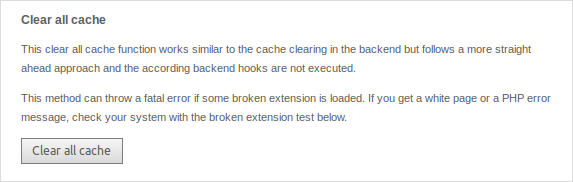
\includegraphics[width=0.9\linewidth]{Images/InstallTool/ClearAllCache.png}
			\end{figure}
		\end{column}
	\end{columns}

\end{frame}

% ------------------------------------------------------------------------------
% Clear All Cache
% ------------------------------------------------------------------------------

\begin{frame}[fragile]
	\frametitle{Install Tool}
	\framesubtitle{Vider tous les caches (2)}

	Actions effectuées quand vous exécutez « Clear all cache » :

	\begin{enumerate}
		\item Le contenu du répertoire \texttt{typo3temp/Cache} est effacé
		\item Les tables \texttt{cf\_*} sont vidées
		\item Les fichiers \texttt{ext\_localconf.php} et \texttt{ext\_tables.php}\newline
			sont chargés depuis les extensions
		\item \texttt{flushCaches()} sont exécutées
	\end{enumerate}

\end{frame}

% ------------------------------------------------------------------------------
% Check For Broken Extensions
% ------------------------------------------------------------------------------

\begin{frame}[fragile]
	\frametitle{Install Tool}
	\framesubtitle{Vérification des extensions endommagées}

	\begin{itemize}
		\item Une nouvelle fonction sous « Important actions » permet aux utilisateurs de vérifier si toutes les extensions peuvent être chargées sans endommager le système
		\item Très utile en cas de mise à jour de la version de TYPO3 4.5 vers 6.2
	\end{itemize}

	\begin{columns}[T]
		\begin{column}{.3\textwidth}
			\begin{figure}\vspace*{-0.4cm}
				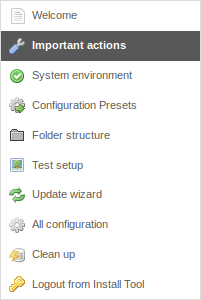
\includegraphics[width=0.7\linewidth]{Images/InstallTool/ImportantActions.png}
			\end{figure}
		\end{column}
		\begin{column}{.7\textwidth}
			\begin{figure}\vspace*{-0.4cm}
				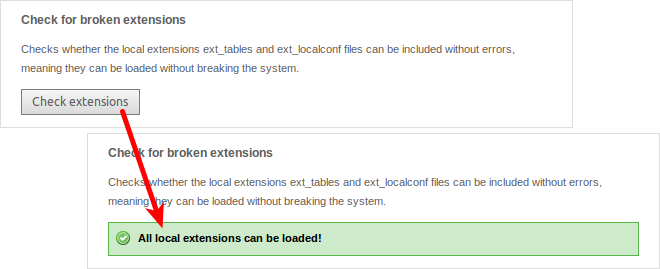
\includegraphics[width=1\linewidth]{Images/InstallTool/CheckForBrokenExtensions.png}
			\end{figure}
		\end{column}
	\end{columns}

\end{frame}

% ------------------------------------------------------------------------------
% Increased Security: Salted Passwords
% ------------------------------------------------------------------------------

\begin{frame}[fragile]
	\frametitle{Install Tool}
	\framesubtitle{Mots de passe salés}

	\begin{itemize}
		\item A la création d'un nouvel administrateur Backend par l'Install Tool, un mot de passe \textbf{salé} est utilisé (nécessite l'installation, le chargement et la configuration de l'extension « saltedpasswords »)\normalsize
		\item L'Install Tool utilise aussi un mot de passe \textbf{salé} (les hash MD5 existants sont automatiquement convertis à la première connexion)\normalsize
	\end{itemize}

	\begin{columns}[T]
		\begin{column}{.3\textwidth}
			\begin{figure}\vspace*{-0.4cm}
				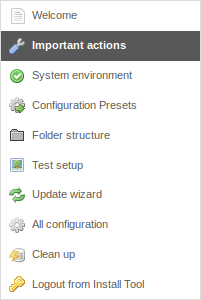
\includegraphics[width=0.7\linewidth]{Images/InstallTool/ImportantActions.png}
			\end{figure}
		\end{column}
		\begin{column}{.7\textwidth}
			\begin{figure}\vspace*{-0.4cm}
				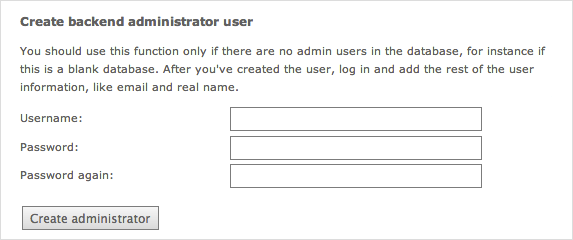
\includegraphics[width=0.9\linewidth]{Images/InstallTool/SaltedPasswords.png}
			\end{figure}
		\end{column}
	\end{columns}

\end{frame}

% ------------------------------------------------------------------------------
% Application Context
% ------------------------------------------------------------------------------

\begin{frame}[fragile]
	\frametitle{Install Tool}
	\framesubtitle{Contexte de l'application}

	\begin{itemize}
		\item La version TYPO3 >= 6.2 prend en compte \textbf{le contexte de l'application}\newline
			\smaller(backporté de TYPO3 Flow)\normalsize
		\item La variable d'environnement \texttt{TYPO3\_CONTEXT} définit le contexte\newline
			\smaller(Par défaut : \texttt{Production}, un sous-contexte tel que \texttt{Production/Staging} est aussi possible)\normalsize

			\begin{lstlisting}
				# File: .htaccess
				# Rules to set Application Context based on hostname:

				RewriteCond %{HTTP_HOST} ^dev\.example\.com$
				RewriteRule (.*) $1 [E=TYPO3_CONTEXT:Development]
				RewriteCond %{HTTP_HOST} ^www\.example\.com$
				RewriteRule (.*) $1 [E=TYPO3_CONTEXT:Production]

				# Sets an environment variable, which is then available to TYPO3 CMS:
				SetEnv TYPO3_CONTEXT Production
			\end{lstlisting}

	\end{itemize}

\end{frame}

% ------------------------------------------------------------------------------
% Application Context
% ------------------------------------------------------------------------------

\begin{frame}[fragile]
	\frametitle{Install Tool}
	\framesubtitle{Pré-paramétrages de TYPO3\_CONF\_VAR}

	\begin{columns}[T]
		\begin{column}{.5\textwidth}

			\begin{itemize}
				\item Certains paramètres TYPO3\_CONF\_VAR peuvent être configurés dans l'Install Tool
				\item Paramètres tels que « debug output », « deprecation log », « devIPmask »
				\item Contextes pré-paramétrés : « Production » et « Développement » (une configuration manuelle et sur mesure est aussi possible)
			\end{itemize}

		\end{column}
		\begin{column}{.5\textwidth}

			\begin{figure}\vspace*{-0.4cm}
				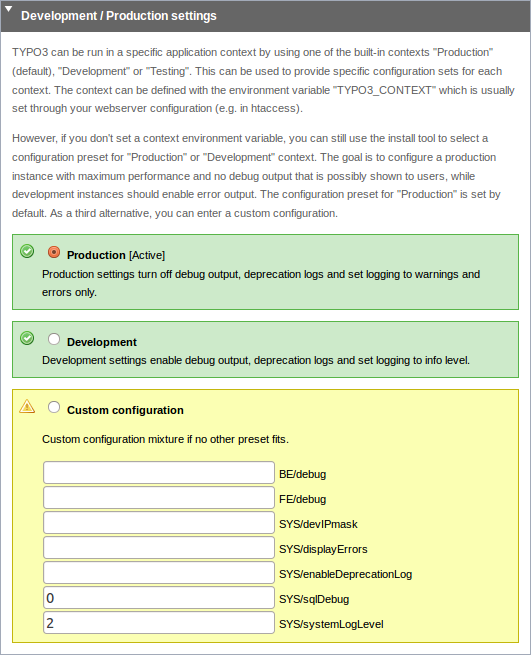
\includegraphics[width=0.8\linewidth]{Images/InstallTool/ApplicationContext.png}
			\end{figure}

		\end{column}
	\end{columns}

\end{frame}

% ------------------------------------------------------------------------------
% Improved Usability
% ------------------------------------------------------------------------------

\begin{frame}[fragile]
	\frametitle{Install Tool}
	\framesubtitle{Utilisabilité améliorée}

	\begin{columns}[T]
		\begin{column}{.5\textwidth}

			\begin{itemize}
				\item Position fixe du menu de gauche lors du déroulement vertical
					\begingroup\color{typo3red}\textbf{(1)}\endgroup
				\item Position fixe du bouton « Write configuration » en bas
					\begingroup\color{typo3red}\textbf{(2)}\endgroup
				\item Regroupement et tri des éléments par section dans « All Configuration » (Ouverture par clic sur le titre de section)
			\end{itemize}

		\end{column}
		\begin{column}{.5\textwidth}

			\begin{figure}\vspace*{-0.4cm}
				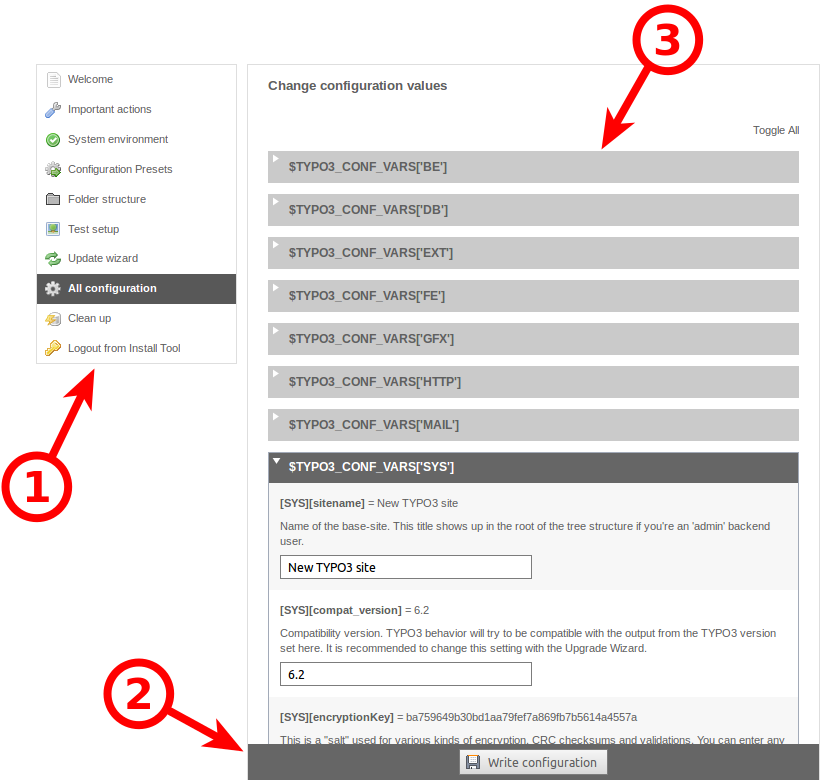
\includegraphics[width=0.8\linewidth]{Images/InstallTool/ImprovedUsability.png}
			\end{figure}

		\end{column}
	\end{columns}

\end{frame}

% ------------------------------------------------------------------------------
% Human-Friendly Error Codes
% ------------------------------------------------------------------------------

\begin{frame}[fragile]
	\frametitle{Install Tool}
	\framesubtitle{Codes d'erreur compréhensibles}

	\begin{itemize}
		\item Des mots-clés compréhensibles peuvent être utilisés dans les options suivantes :\newline
			(Pour TYPO3 < 6.2, seules des valeurs numériques étaient possibles)
	\end{itemize}

	\begin{columns}[T]
		\begin{column}{.4\textwidth}
			\advance\leftskip+0.8cm

			\smaller
				\texttt{[SYS][errorHandlerErrors]}\newline
				\texttt{[SYS][exceptionalErrors]}\newline
				\texttt{[SYS][syslogErrorReporting]}\newline
				\texttt{[SYS][belogErrorReporting]}\newline
			\normalsize

		\end{column}
		\begin{column}{.6\textwidth}

			\begin{figure}\vspace*{-0.4cm}
				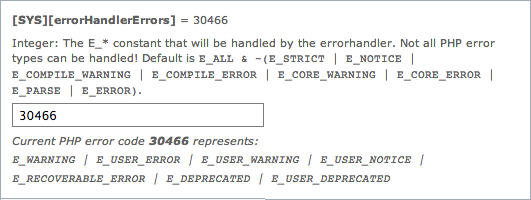
\includegraphics[width=0.9\linewidth]{Images/InstallTool/HumanFriendlyErrorCodes.png}
			\end{figure}

		\end{column}
	\end{columns}

	\vspace{0.2cm}

	\begin{itemize}
		\item Un ViewHelper ExtBase \textbf{format.phpErrorCode} s'occupe de la conversion des codes d'erreur PHP
	\end{itemize}

\end{frame}

% ------------------------------------------------------------------------------
% Errors In Folder Structure
% ------------------------------------------------------------------------------

\begin{frame}[fragile]
	\frametitle{Install Tool}
	\framesubtitle{Erreurs dans la structure des dossiers}

	\begin{itemize}
		\item Le nombre d'erreurs sous « Folder Structure » est signalé par un badge (nombre sur rond rouge)
	\end{itemize}

	\begin{figure}
		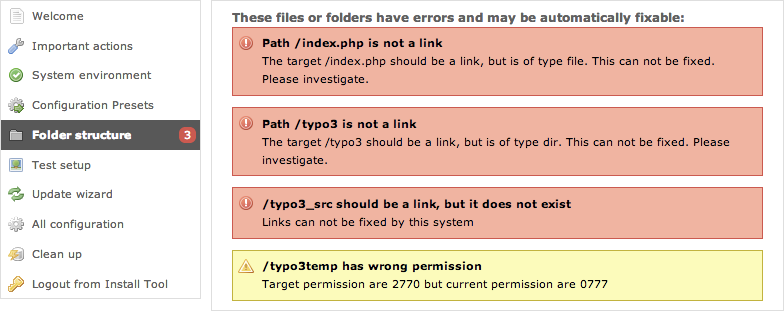
\includegraphics[width=0.95\linewidth]{Images/InstallTool/ErrorsInFolderStructure.png}
	\end{figure}

\end{frame}

% ------------------------------------------------------------------------------
% Core Updates
% ------------------------------------------------------------------------------

\begin{frame}[fragile]
	\frametitle{Install Tool}
	\framesubtitle{Mises à jour du cœur}

	\begin{itemize}
		\item Mise à jour du cœur dans sa dernière version mineure en un clic 
		\item La variable d'environnement \texttt{TYPO3\_DISABLE\_CORE\_UPDATER=1} désactive cette fonctionnalité
	\end{itemize}

	\begin{figure}
		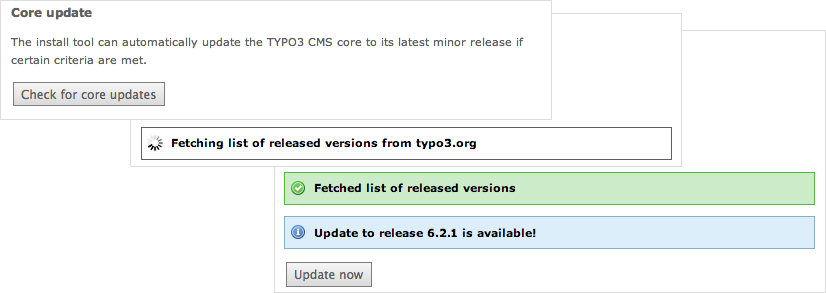
\includegraphics[width=0.95\linewidth]{Images/InstallTool/CoreUpdate.png}
	\end{figure}

\end{frame}

% ------------------------------------------------------------------------------
% Miscellaneous
% ------------------------------------------------------------------------------

\begin{frame}[fragile]
	\frametitle{Install Tool}
	\framesubtitle{Divers (1)}

	\begin{itemize}
		\item Tous les formulaires sont protégés des CSRF (\textit{cross-site request forgery})
		\item L'Install Tool utilise une version simplifié du « Fluid Standalone View »
		\item Seules les fonctions essentielles de TYPO3 sont chargées\newline
			(Si le fichier \texttt{ext\_localconf.php} ou le fichier \texttt{ext\_tables.php} est corrompu, il ne peut plus endommager l'Install Tool)
		\item Nouvelle URL : \tabto{2.6cm} \texttt{typo3/sysext/install/Start/Install.php}\newline
			Versions précédentes :\newline
			\texttt{typo3/install/index.php}\newline
			(la redirection de l'ancienne URL à la nouvelle est automatique)
		\item La désactivation du cache permet à l'Install Tool de rester utilisable, même si le cache présente du code PHP invalide
	\end{itemize}

\end{frame}

% ------------------------------------------------------------------------------
% Miscellaneous
% ------------------------------------------------------------------------------

\begin{frame}[fragile]
	\frametitle{Install Tool}
	\framesubtitle{Divers (2)}

	\begin{itemize}
		\item Vérification de l'option PHP \texttt{xdebug.max\_nesting\_level} avec une valeur de 250 ou plus (la valeur par défaut « 100 » peut poser problème)
		\item « Relaxed permission check » :

			\small
				Si le dossier Web ne dispose pas des permissions appropriées (par exemple « 2770 »)
				et que cela ne peut être corrigé (par exemple parce que le répertoire ne dépend pas
				de l'utilisateur système utilisé pour l'Install Tool), la première étape de l'installation
				ne fonctionne pas.
				L'option « targetPermissionRelaxed » abaisse le niveau de contrôle et permet de poursuivre l'installation tant que les sous-dossiers peuvent être créés.
			\normalsize

	\end{itemize}

\end{frame}

% ------------------------------------------------------------------------------
% Miscellaneous
% ------------------------------------------------------------------------------

\begin{frame}[fragile]
	\frametitle{Install Tool}
	\framesubtitle{Divers (3)}

	\begin{itemize}
		\item Options enlevées (keys) de l'Install Tool\newline
			\small(et donc aussi du fichier \texttt{LocalConfiguration.php}) :\normalsize
	\end{itemize}

	\begin{columns}[T]
		\begin{column}{.5\textwidth}
			\advance\leftskip+0.8cm
			\smaller
				\texttt{BE/loginLabels}\newline
				\texttt{BE/loginNews}\newline
				\texttt{BE/useOnContextMenuHandler}\newline
				\texttt{EXT/em\_mirrorListURL}\newline
				\texttt{EXT/em\_wsdlURL}\newline
				\texttt{EXT/extList}\newline
				\texttt{EXT/extList\_FE}\newline
				\texttt{EXT/noEdit}\newline
			\normalsize
		\end{column}
		\begin{column}{.5\textwidth}
			\smaller
				\texttt{FE/defaultTypoScript\_editorcfg}\newline
				\texttt{FE/simulateStaticDocuments}\newline
				\texttt{GFX/noIconProc}\newline
				\texttt{GFX/TTFLocaleConv}\newline
				\texttt{SYS/additionalAllowedClassPrefixes}\newline
				\texttt{SYS/caching/cacheBackends}\newline
				\texttt{SYS/caching/cacheFrontends}\newline
				\texttt{SYS/extCache}\newline
				\texttt{SYS/T3instID}\newline
			\normalsize
		\end{column}

	\end{columns}

\end{frame}

% ------------------------------------------------------------------------------

